\documentclass[12pt, a4paper]{article}
\usepackage[utf8]{inputenc}
\usepackage[english]{babel}
\usepackage{fancyhdr}
\usepackage{datetime}
\usepackage{hyperref}
\usepackage{longtable}
\usepackage{graphicx}
\usepackage{listings}
\usepackage{xcolor}
\lstset { %
    language=C++,
    backgroundcolor=\color{black!5}, % set backgroundcolor
    basicstyle=\footnotesize,% basic font setting
    keywordstyle=\color{blue}\ttfamily,
    stringstyle=\color{red}\ttfamily,
    commentstyle=\color{green}\ttfamily,
    morecomment=[l][\color{magenta}]{\#}
}
\usepackage[font=small,labelfont=bf]{caption}
\hypersetup{
    colorlinks,
    citecolor=black,
    filecolor=black,
    linkcolor=black,
    urlcolor=black
}

\def\labelitemi{--}
\setcounter{tocdepth}{3}
\pagestyle{fancy}
\fancyhf{}
\renewcommand{\headrulewidth}{1pt}
\renewcommand{\footrulewidth}{1pt}
\rhead{\leftmark}
\rfoot{Page \thepage}

\begin{document}

\begin{titlepage}

    \newcommand{\HRule}{\rule{\linewidth}{0.5mm}} % Defines a new command for the horizontal lines, change thickness here
    
    \center % Center everything on the page
     
    %----------------------------------------------------------------------------------------
    %	HEADING SECTIONS
    %----------------------------------------------------------------------------------------
    
    \textsc{\LARGE Università Degli Studi Di Milano}\\[1.5cm] % Name of your university/college
    \textsc{\Large Real-Time Graphics Programming}\\[0.5cm] % Major heading such as course name
    %\textsc{\large Assignment 1}\\[0.5cm] % Minor heading such as course title
    
    %----------------------------------------------------------------------------------------
    %	TITLE SECTION
    %----------------------------------------------------------------------------------------
    
    \HRule \\[0.4cm]
    { \huge \bfseries Real-time autostereogram rendering pipeline }\\[0.4cm] % Title of your document
    \HRule \\[1.5cm]
     
    %----------------------------------------------------------------------------------------
    %	AUTHOR SECTION
    %----------------------------------------------------------------------------------------
    
    \begin{minipage}{0.4\textwidth}
    \begin{flushleft} \large
    \emph{Author:}\\
    Giovanni \textsc{Cocco} \\
    \end{flushleft}
    \end{minipage}
    ~
    \begin{minipage}{0.4\textwidth}
    \begin{flushright} \large
    \emph{Academic year:} \\
    2022-2023\\
    \end{flushright}
    \end{minipage}\\[2cm]
    
    % If you don't want a supervisor, uncomment the two lines below and remove the section above
    %\Large \emph{Author:}\\
    %John \textsc{Smith}\\[3cm] % Your name
    
    %----------------------------------------------------------------------------------------
    %	DATE SECTION
    %----------------------------------------------------------------------------------------
    
    {\large \today}\\[4cm] % Date, change the \today to a set date if you want to be precise
    
    %----------------------------------------------------------------------------------------
    %	LOGO SECTION
    %----------------------------------------------------------------------------------------
    
    
\includegraphics[width=130px, keepaspectratio]{img/unimi.png}\\[1cm] % Include a department/university logo - this will require the graphicx package
     
    %----------------------------------------------------------------------------------------
    
    \vfill % Fill the rest of the page with whitespace
    
    \end{titlepage}

\clearpage
\tableofcontents{}
\listoffigures
\listoftables
\lstlistoflistings
\clearpage

\section{Abstract}
In this document we discuss the algorithms, the choices and the implementation details of a real-time autostereogram rendering pipeline built with OpenGL 4.3.\\\\
The pipeline presented allow the rendering of autostereograms starting from a depth buffer that is always produces
as a result on all classical rasterization rendering algorithms. More elaborated effect can be achieved if we supply as input also the color buffer and 
the normal buffer.\\\\
We will first briefly explain what an autostereogram is and how it works from a psychological point of view. We will then discuss a general algorithm to create them.
We will then discuss the implementation detail of the project.\\\\
It should be noted that the input needed for the autostereogram generation algorithm are produced as a result of most real-time rendering pipeline and this 
mean that is possible to apply this technique to an already existent rendering pipeline.\\\\
For this project we made a simple rendering pipeline using Blinn-Phong illumination model, as we will see more sophisticated model give little gain in 
the final result.\\\\
The project also implements blend skinning for skeletal animation, we will discuss the implementation and the difference between linear blend skinning and
dual quaternion skinning.\\\\
We will see how the performance of this pipeline can be totally in the frame budget on most GPU buy may suffer on old laptop one while still
providing 60 frames per second.

\clearpage
\section{Autostereogram}
\subsection{What is an autostereogram}
A stereogram is a 2D image that creates the optical illusion of a 3D scene\footnote{https://en.wikipedia.org/wiki/Autostereogram}. Autostereograms are a particular kind of stereograms
that create this illusion without requiring any additional equipment.\\\\
Our brain is able to perceive depth because each eye receives a different image because they are in slightly different positions on one's head.
We can exploit this behavior by producing one image with repeating patter causing and object to be in the right position from the point of view of each eye
if the eye separation of the subject is the correct one.\\\\
Note that it might take some practice before being able to control the eye separation and be able to see
the optical illusion. For more information on some viewing technique one may take a look at: \url{https://www.hidden-3d.com/how_to_view_stereogram.php}.\\\\
\begin{center}
    \centering
    
\includegraphics[width=1.0\textwidth]{img/shark.png}
    \captionof{figure}{Autostereogram of a shark}
\end{center}
\clearpage
\subsection{Autostereogram rendering algorithm}
To render an autostereogram we need first to understand the underling geometry.\\
\begin{center}
    \centering
    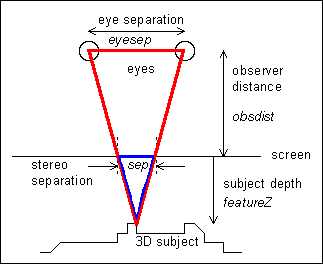
\includegraphics[width=0.7\textwidth]{img/geometry.png}
    \captionof{figure}{The geometry of an autostereogram}
\end{center}
If the two points where the line of sight intercept the screen have the same color the depth of the 3D
subject will be perceived.\\\\
As we can see from the figure the two highlighted triangles have the same angles and as such they are similar.
This means they are proportional, and so we can calculate the separation with the following equation.
\[
sep = \frac{eyesep \cdot featureZ}{featureZ + obsdist}
\]
The general method to create an autostereogram is the following\footnote{http://www.techmind.org/stereo/stech.html}:
\begin{itemize}
    \item Create a depth map of the scene.
    \item For each horizontal line, moving from left to right, and for each point of the depth map link together all the pixel that will have the same color.
    \item Assign to each point a random color making sure the linked one will have the same.
\end{itemize}

\subsection{Advanced effects}
The choice of which color assign to a pixel allow for different effect.\\\\
It is possible to use a completely random color, but is also possible use a texture pattern that will be repeated horizontally.\\\\
It is also possible to highlight the edge of the objects or using a color based on the real object color.
\begin{center}
    \centering
    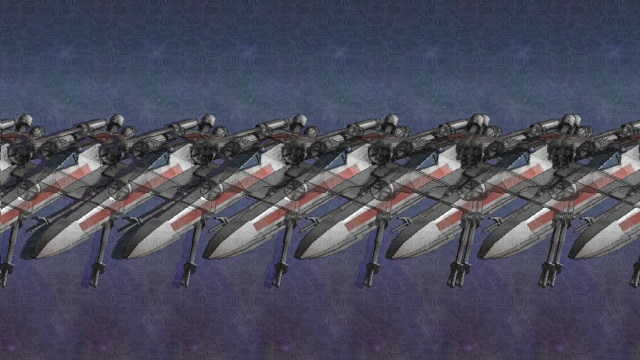
\includegraphics[width=1.0\textwidth]{img/ship.png}
    \captionof{figure}{Object color are used}
\end{center}
As one may expect this means objects will bleed horizontally to other pixels in a repeating fashion.
\section{Scene management}
\subsection{Handle multiple scenes}
The project requires different scenes to be loaded when selected from the GUI.\\\\
To achieve this the class \textbf{SceneManager} is responsible for loading the correct scene and unloading the old one
freeing any no longed used resources.\\\\
The \textbf{SceneManager} class hold a polymorphic pointer to a class \textbf{Scene}, when asked to load a new one
the current one is deleted and the old one is instanced creating a subclass of type \textbf{Scene}.\\\\
This mean there is a subclass of \textbf{Scene} for every scene in the project. This method in general does not
scale well, but for a project of this scale loading a scene specification from an asset file was considered overengineering.
It should be noted that if the scene was loaded from a file we could not use the polymorphic nature of the class
\textbf{Scene} to override its method \textbf{Update}. In this situation we would be required to support scripting in the
scene with something like Lua, again this was considered overengineer.\\\\
The constructor of \textbf{Scene} will load the required assets as we will discuss later. This requires up to 40MB of 
data to be loaded from the disk on demand. As this require quite some time the class \textbf{SceneManager} also
hold an instance to an object of type \textbf{LoadingScreen} that will create a simple loading screen before calling
the \textbf{Scene} constructor.
\begin{center}
    \centering
    
\includegraphics[width=1.0\textwidth]{img/loading.png}
    \captionof{figure}{Loading screen}
\end{center}
The \textbf{LoadingScreen} constructor will create the shader, the quad and the texture needed for the loading screen
rendering.\\\\
The quad is simply a square with x, y coordinate with values in -1, 1. To ensure the loading screen will be rendered correctly
in any aspect rateo the inverse of the rateo is passed to the vertex shader as a uniform called \textbf{rateo}.\\\\
The vertex shader will draw the quad as high as the screen and center horizontally.
\begin{lstlisting}[caption={Loading screen vertex shader},captionpos=b]
#version 430 core
layout (location = 0) in vec3 position;
uniform float rateo;
    
out vec2 uv;
void main() {
    uv = vec2(0.5)+position.xy*0.5;
    vec4 pos = vec4(position, 1.0);
    pos.x *= rateo;
    uv.y = -uv.y;
    gl_Position = pos;
}
\end{lstlisting}
To hide the missing part on right and left
the buffer was cleared with \textbf{glClear} with the clear color set as the loading screen image background color.\\\\
The \textbf{SceneManager} also forward the call to the method process to the current loaded scene to allow the scene
to be updated with the current \textbf{deltaTime}.

\subsection{Assets loading}
\textbf{Scene} constructor will set the camera position, the light direction, the skybox, load all the required models and texture
and set all the object in the scene with the correct position and orientation.\\\\
Models and textures are loaded into two different \textbf{std::vector} and only their pointer are stored in the object struct.
This allows to load shader models and textures only once.\\\\
\textbf{Assimp} was used to load models and \textbf{stb\_image} to load textures. Both these code path
reused the code written by Prof. Davide Gadia which was showed during lab lectures.

\subsection{Object struct}
Every object is the scene is of type \textbf{Object} that also hold material properties for the Blinn-Phong lighting model.
\begin{lstlisting}[caption={Object struct},captionpos=b]
struct Object {
    glm::vec3 position = glm::vec3(0.0, 0.0, 0.0);
    glm::vec3 rotation = glm::vec3(0.0, 0.0, 0.0);
    glm::vec3 scale = glm::vec3(1.0, 1.0, 1.0);

    Model *model;
    GLuint texture;
    GLfloat alphaMultiplier = 1.0;

    glm::vec3 specularColor = glm::vec3(1.0);
    float shininess = 500.0;
    float diffuseFactor = 1.0;
    float specularFactor = 0.4;
};
\end{lstlisting}
The rotation is expressed as Euler angles. This is not the best representation for rotation in video games and quaternion
give simpler cumulation and interpolation formulas. Euler angles was preferred for their easier setup without a visual
scene editor, again to avoid unneeded overengineering.\\\\
The float \textbf{alphaMultiplier} is a special value that affect the alpha component of the fragment.
This is used for some advanced effect during the stereogram rendering and will be discussed later.\\\\
Skinned Object are a subclass Object holding the skinned model and the animator. Note that in C++ struct and class
are basically the same thing as the only difference is that by default struct members are public, whereas they are private in classes.
\begin{lstlisting}[caption={SkinnedObject struct},captionpos=b]
struct SkinnedObject : public Object {
    ModelAnimated *s_model;
    Animator *anim;
};
\end{lstlisting}

\subsection{Camera and input processing}
Camera and input management is based on code written during lab lectures. The \textbf{SceneCamera} class contains
an object of type \textbf{Camera} as it was written during the lab lectures.\\\\
As only the camera is affected by user input, beside GUI, the \textbf{SceneCamera} class also manage the input
using the \textbf{glfw} library.\\\\
The \textbf{SceneCamera} camera is created by the \textbf{SceneManager} and passed to the \textbf{Scene} on
their creation. This not only reduce unneeded object creation and destruction, but most importantly this allows
the constructor of \textbf{SceneCamera} to register the \textbf{glfw} callback before \textbf{ImGUI} register its own.
This seems to workarounds a bug with \textbf{ImGUI} from becoming unresponsive when the window lose focus on Linux.  

\section{GUI}
The GUI menus was build with \textbf{ImGUI}. The class \textbf{GUI} is responsable for creating and destroying the
\textbf{ImGUI} context as well as render all the GUI when the method \textbf{RenderMenu} is called.
\begin{center}
    \centering
    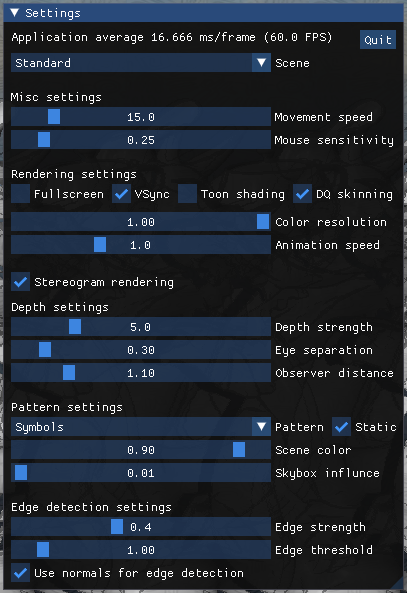
\includegraphics[width=0.6\textwidth]{img/gui.png}
    \captionof{figure}{Settings GUI}
\end{center}
The variables affected by the GUI are placed in a struct \textbf{Context} that is created in the \textbf{main} and
passed as a pointer to most objects in the application. This avoids proliferation of global variables for data 
that need to be shader by multiple objects.

\section{Rendering}
\subsection{Illumination model}

\subsection{Toon shading}

\subsection{Skybox}

\subsection{Autostereogram}

\section{Skeletal animation}

\subsection{Linear blend skinning}

\subsection{Dual quaternion skinning}

\section{Performance evaluation}

\section{Conclusion}

\end{document}